\noindent
{\Large \textbf{\section{Программирование}}} \par
\noindent
\vspace{-40pt}

{\Large \textbf{\subsection{Заполнение базы данных}}} \par

Код создания таблиц для базы данных приведен в приложении А. Код для генерации данных был написан на языке Python, он приведен в приложении Б. 
Количество записей в сгенерированных таблицах представлено в таблице \ref{kolvo}.

\begin{table}[htbp]
\centering
\label{tab:db_records_count_grid}
\begin{tabular}{|l|r|}
\hline
\textbf{Название таблицы} & \textbf{Количество записей} \\ \hline
exhibit\_materials     & 2 261 727 \\ \hline
passports              &   301 374 \\ \hline
exhibits               &    67 000 \\ \hline
exhibit\_placements    &    12 196 \\ \hline
display\_places        &     2 535 \\ \hline
exhibition\_curators   &        781 \\ \hline
exhibitions            &        200 \\ \hline
employees              &        180 \\ \hline
exhibition\_spaces     &        100 \\ \hline
materials              &         63 \\ \hline
epochs                 &          6 \\ \hline
exhibition\_type       &          6 \\ \hline
exhibition\_subject    &          5 \\ \hline
exhibit\_conditions    &          5 \\ \hline
room\_type             &          4 \\ \hline
humidity\_categories   &          4 \\ \hline
exhibition\_status     &          4 \\ \hline
temp\_categories       &          4 \\ \hline
exhibit\_status        &          4 \\ \hline
lighting\_categories   &          4 \\ \hline
\textbf{ВСЕГО ЗАПИСЕЙ В БД} & \textbf{2 646 202} \\ \hline
\end{tabular}
\caption{Количество записей в таблицах базы данных}
\label{kolvo}
\end{table}

\vspace{-40pt}

{\Large \textbf{\subsection{Запросы}}} \par

Лист проверки выполнения запросов представлен на Рис.\ref{queriesscreen}.

\begin{figure}[H]
    \centering
    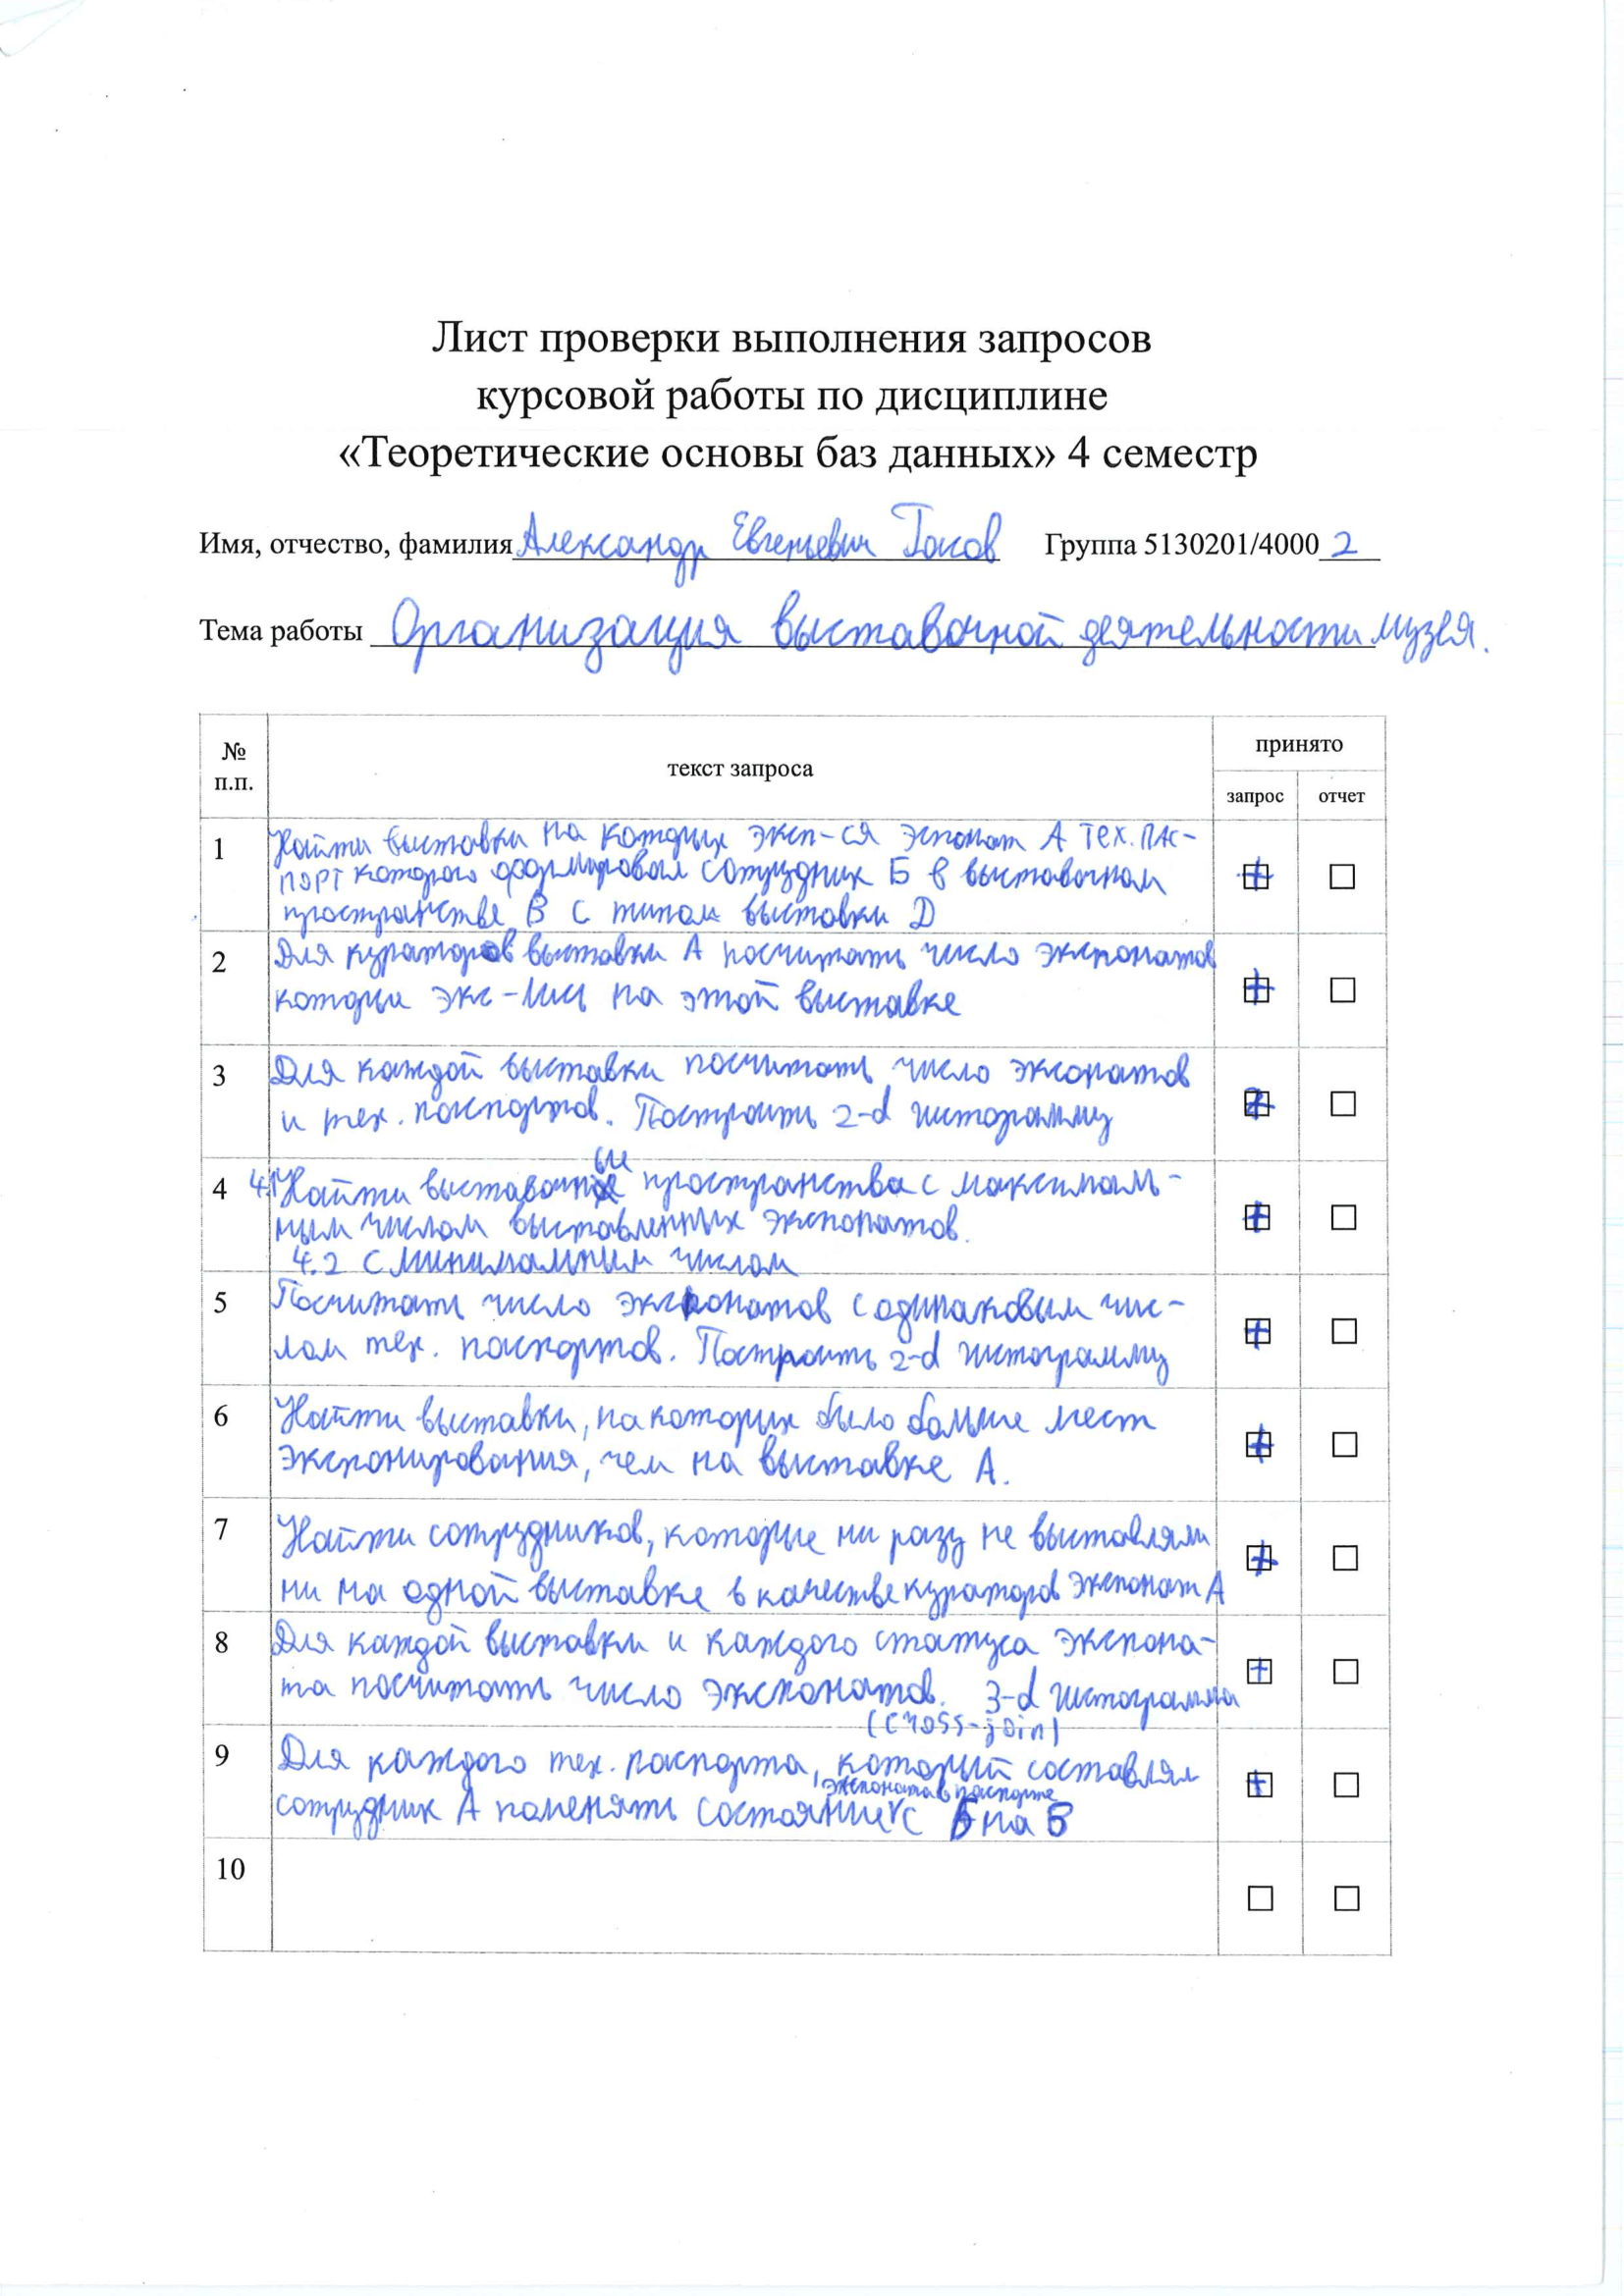
\includegraphics[width=\textwidth,height=0.90\textheight,keepaspectratio]{pic/queriesscreen.png}
    \caption{Лист проверки выполнения запросов}
    \label{queriesscreen}
\end{figure}

Для анализа запросов использовалась команда \texttt{EXPLAIN ANALYZE}. Время планирования и выполнения запросов приведено в таблице~\ref{tab:query-time}. \par

\begin{table}[H]
\centering
{\small
\begin{tabular}{|c|c|c|}
\hline
Запрос  & Planning Time, мс & Execution Time, мс \\
\hline
1 & 0.567 & 17.300 \\
\hline
2 & 0.665 & 12.473 \\
\hline
3 & 0.090 & 41.806 \\
\hline
4.1  & 0.104 & 7.288 \\
\hline
4.2  & 0.281 & 9.731 \\
\hline
5  & 0.095 & 64.808 \\
\hline
6  & 0.067 & 3.646 \\
\hline
7  & 0.174 & 2.170 \\
\hline
8  & 0.129 & 69.868 \\
\hline
9  & 0.062 & 28.464 \\
\hline
\end{tabular}}
\caption{Время планирования и выполнения запросов}
\label{tab:query-time}
\end{table}

Визуализации планов выполнения запросов были построены с помощью
сервиса explain.dalibo.com \cite{site:explain}.

\subsection{Запрос 1}

Найти выставки, на которых экспонируется экспонат А, технический паспорт которого формировал сотрудник Б, в выставочном пространстве В с типом выставки Д. Текст запроса представлен в Листинге~\ref{lst:q1}. \par

\lstinputlisting[language=SQL, caption={Запрос 1}, label={lst:q1}, basicstyle=\ttfamily\footnotesize]{../../../queries/q1.sql}

Реляционная формула запроса:
\[
\begin{gathered}
R_1 = 
\pi_{\text{exhibition\_name}}
\left(
\sigma_{\substack{
\text{exhibit\_name}=A \ \land \\
\text{employee}=B \ \land \\
\text{room\_type\_name}=C \ \land \\
\text{exhibition\_type\_name}=D
}}
\left(
\begin{gathered}
\text{exhibitions} 
\bowtie_{\text{exhibition\_id}} \\
\text{exhibit\_placements} 
\bowtie_{\text{exhibit\_id}} \\
\text{exhibits} 
\bowtie_{\text{exhibit\_id}} \\
\text{passports} 
\bowtie_{\text{employee\_id}} \\
\text{employees} 
\bowtie_{\text{display\_place\_id}} \\
\text{display\_places} 
\bowtie_{\text{exhibition\_space\_id}} \\
\text{exhibition\_spaces} 
\bowtie_{\text{room\_type\_id}} \\
\text{room\_type} 
\bowtie_{\text{exhibition\_type\_id}} \\
\text{exhibition\_type}
\end{gathered}
\right)
\right), \\
\text{где } \bowtie \text{ --- это natural join}
\end{gathered}
\]

Результат выполнения запроса 1 (выведены первые 20 строк) представлен на Рис.\ref{fig:q1-result}. \par

\begin{figure}[H]
    \centering
    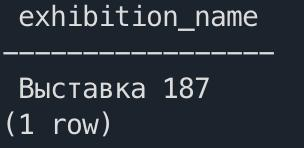
\includegraphics[width=\textwidth,height=3cm,keepaspectratio]{pic/q1.jpg}
    \caption{Результат выполнения запроса 1 (выведены первые 20 строк)}
    \label{fig:q1-result}
\end{figure}

План выполнения запроса 1 представлен на Рис.\ref{fig:q1-explain}. \par

\begin{figure}[H]
    \centering
    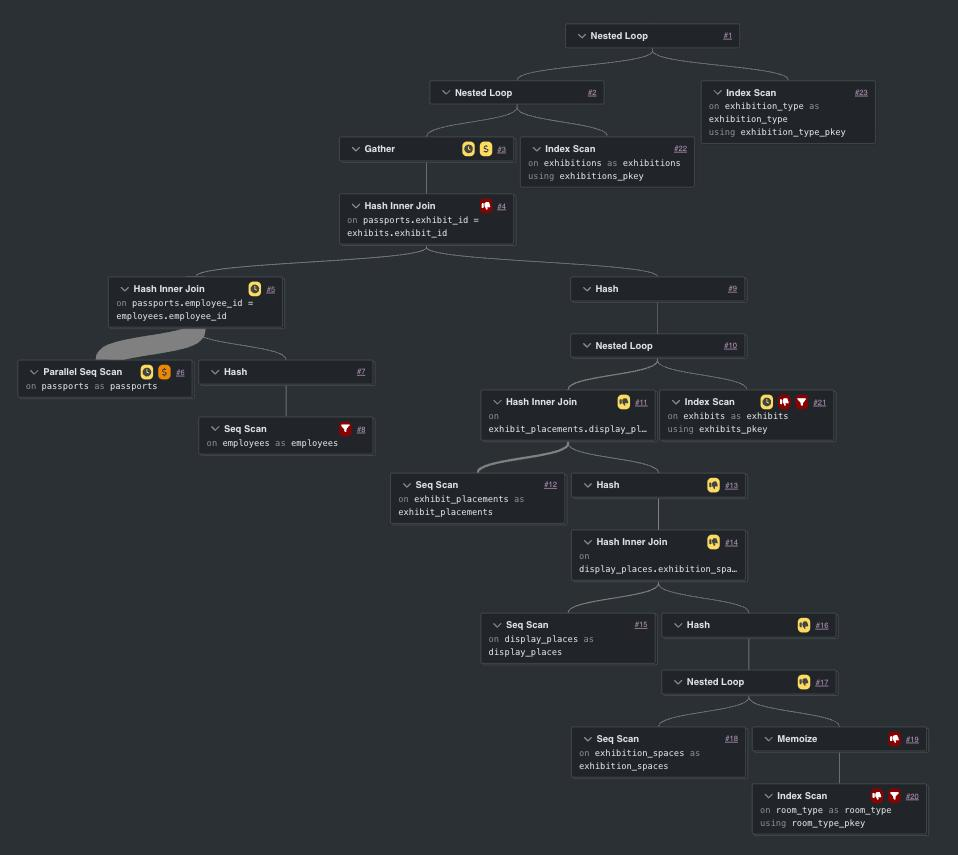
\includegraphics[width=\textwidth,height=0.75\textheight,keepaspectratio]{pic/exp1.jpg}
    \caption{План выполнения запроса 1}
    \label{fig:q1-explain}
\end{figure}

В плане выполнения запроса последовательно соединяются таблицы выставок, размещений, экспонатов, паспортов, сотрудников, мест экспонирования, выставочных пространств, типов помещений и типов выставок. Фильтрация по заданным значениям выполняется после получения связанных строк, а итоговая operation возвращает только название подходящей выставки. \par

\subsection{Запрос 2}

Для кураторов выставки А посчитать число экспонатов, которые экспонировались на этой выставке. Текст запроса представлен в Листинге~\ref{lst:q2}. \par

\lstinputlisting[language=SQL, caption={Запрос 2}, label={lst:q2}, basicstyle=\ttfamily\footnotesize]{../../../queries/q2.sql}

Реляционная формула запроса:
\[
\begin{gathered}
R_2 = 
\gamma_{\substack{\text{first\_name}, \text{last\_name}; \\ \text{COUNT}(\text{distinct } \text{exhibit\_id})}}
\left(
\sigma_{\text{exhibition\_name}=A}
\left(
\begin{gathered}
\text{employees} 
\bowtie_{\text{employee\_id}} \\
\text{exhibition\_curators} 
\bowtie_{\text{exhibition\_id}} \\
\text{exhibitions} 
\bowtie_{\text{employee\_id}} \\
\text{passports} 
\bowtie_{\text{exhibit\_id}} \\
\text{exhibits} 
\bowtie_{\substack{\text{exhibit\_id} \\ \text{exhibition\_id}}} \\
\text{exhibit\_placements}
\end{gathered}
\right)
\right), \\
\text{где } \bowtie \text{ --- это natural join}
\end{gathered}
\]

Результат выполнения запроса 2 (выведены первые 20 строк) представлен на Рис.\ref{fig:q2-result}. \par

\begin{figure}[H]
    \centering
    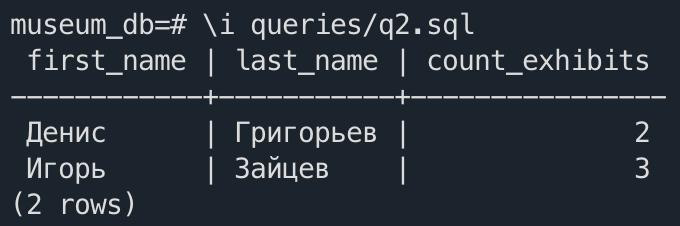
\includegraphics[width=\textwidth,height=3cm,keepaspectratio]{pic/q2.jpg}
    \caption{Результат выполнения запроса 2 (выведены первые 20 строк)}
    \label{fig:q2-result}
\end{figure}

План выполнения запроса 2 представлен на Рис.\ref{fig:q2-explain}. \par

\begin{figure}[H]
    \centering
    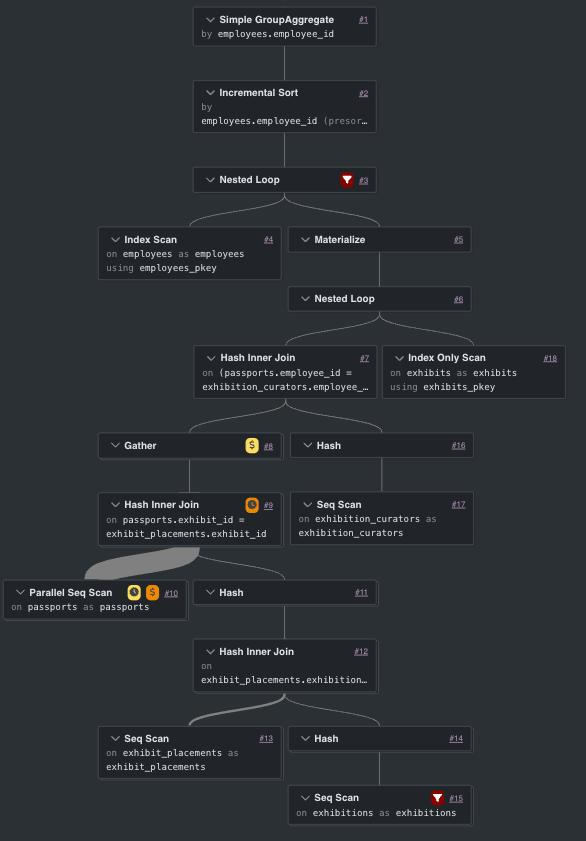
\includegraphics[width=\textwidth,height=0.9\textheight,keepaspectratio]{pic/exp2.jpg}
    \caption{План выполнения запроса 2}
    \label{fig:q2-explain}
\end{figure}

План сначала отбирает заданную выставку, затем соединяет ее с кураторами, сотрудниками, паспортами, экспонатами и размещениями. После соединений выполняется группировка по сотруднику и подсчет различных экспонатов, относящихся к выбранной выставке. \par

\subsection{Запрос 3}

Для каждой выставки посчитать число экспонатов и технических паспортов. Текст запроса представлен в Листинге~\ref{lst:q3}. \par

\lstinputlisting[language=SQL, caption={Запрос 3}, label={lst:q3}, basicstyle=\ttfamily\footnotesize]{../../../queries/q3.sql}

Реляционная формула запроса:
\[
\begin{gathered}
R_3 = 
\gamma_{\substack{\text{exhibition\_id}, \text{exhibition\_name}; \\ \text{COUNT}(\text{distinct } \text{exhibit\_id}), \\ \text{COUNT}(\text{distinct } \text{passport\_id})}}
\left(
\begin{gathered}
\text{exhibitions}
\bowtie(left)_{\text{exhibition\_id}} \\
\text{exhibit\_placements}
\bowtie(left)_{\text{exhibit\_id}} \\
\text{passports}
\end{gathered}
\right), \\
\text{где } \bowtie \text{ --- это natural join}
\end{gathered}
\]

Результат выполнения запроса 3 (выведены первые 20 строк) представлен на Рис.\ref{fig:q3-result}. \par

\begin{figure}[H]
    \centering
    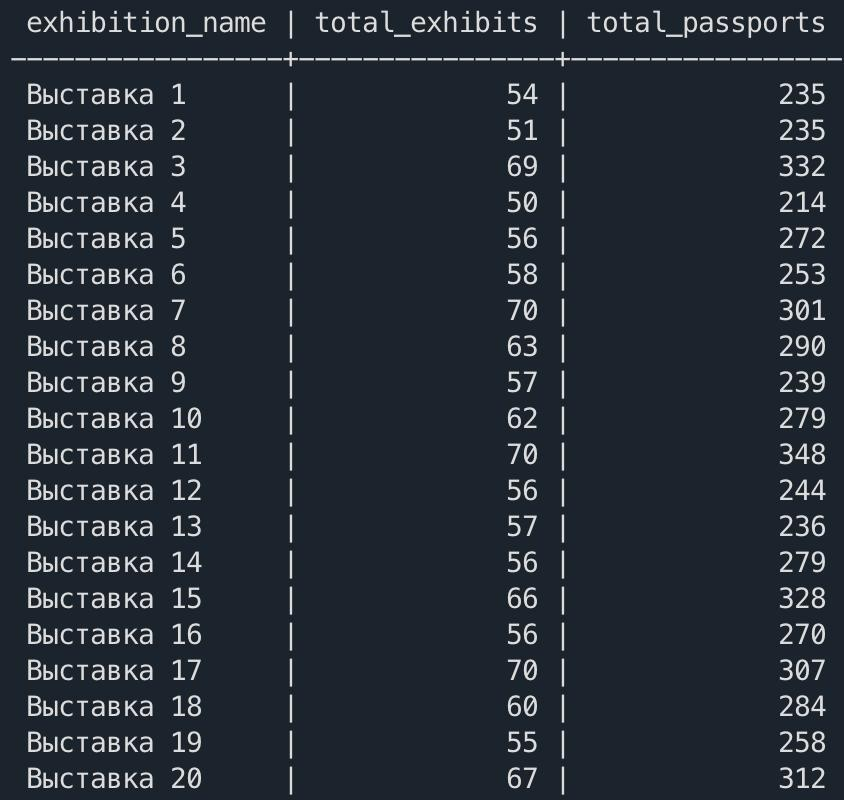
\includegraphics[width=\textwidth,height=8cm,keepaspectratio]{pic/q3.jpg}
    \caption{Результат выполнения запроса 3 (выведены первые 20 строк)}
    \label{fig:q3-result}
\end{figure}

Двумерная гистограмма, построенная по результатам запроса 3, представлена на Рис.\ref{fig:q3-histogram}. \par

\begin{figure}[H]
    \centering
    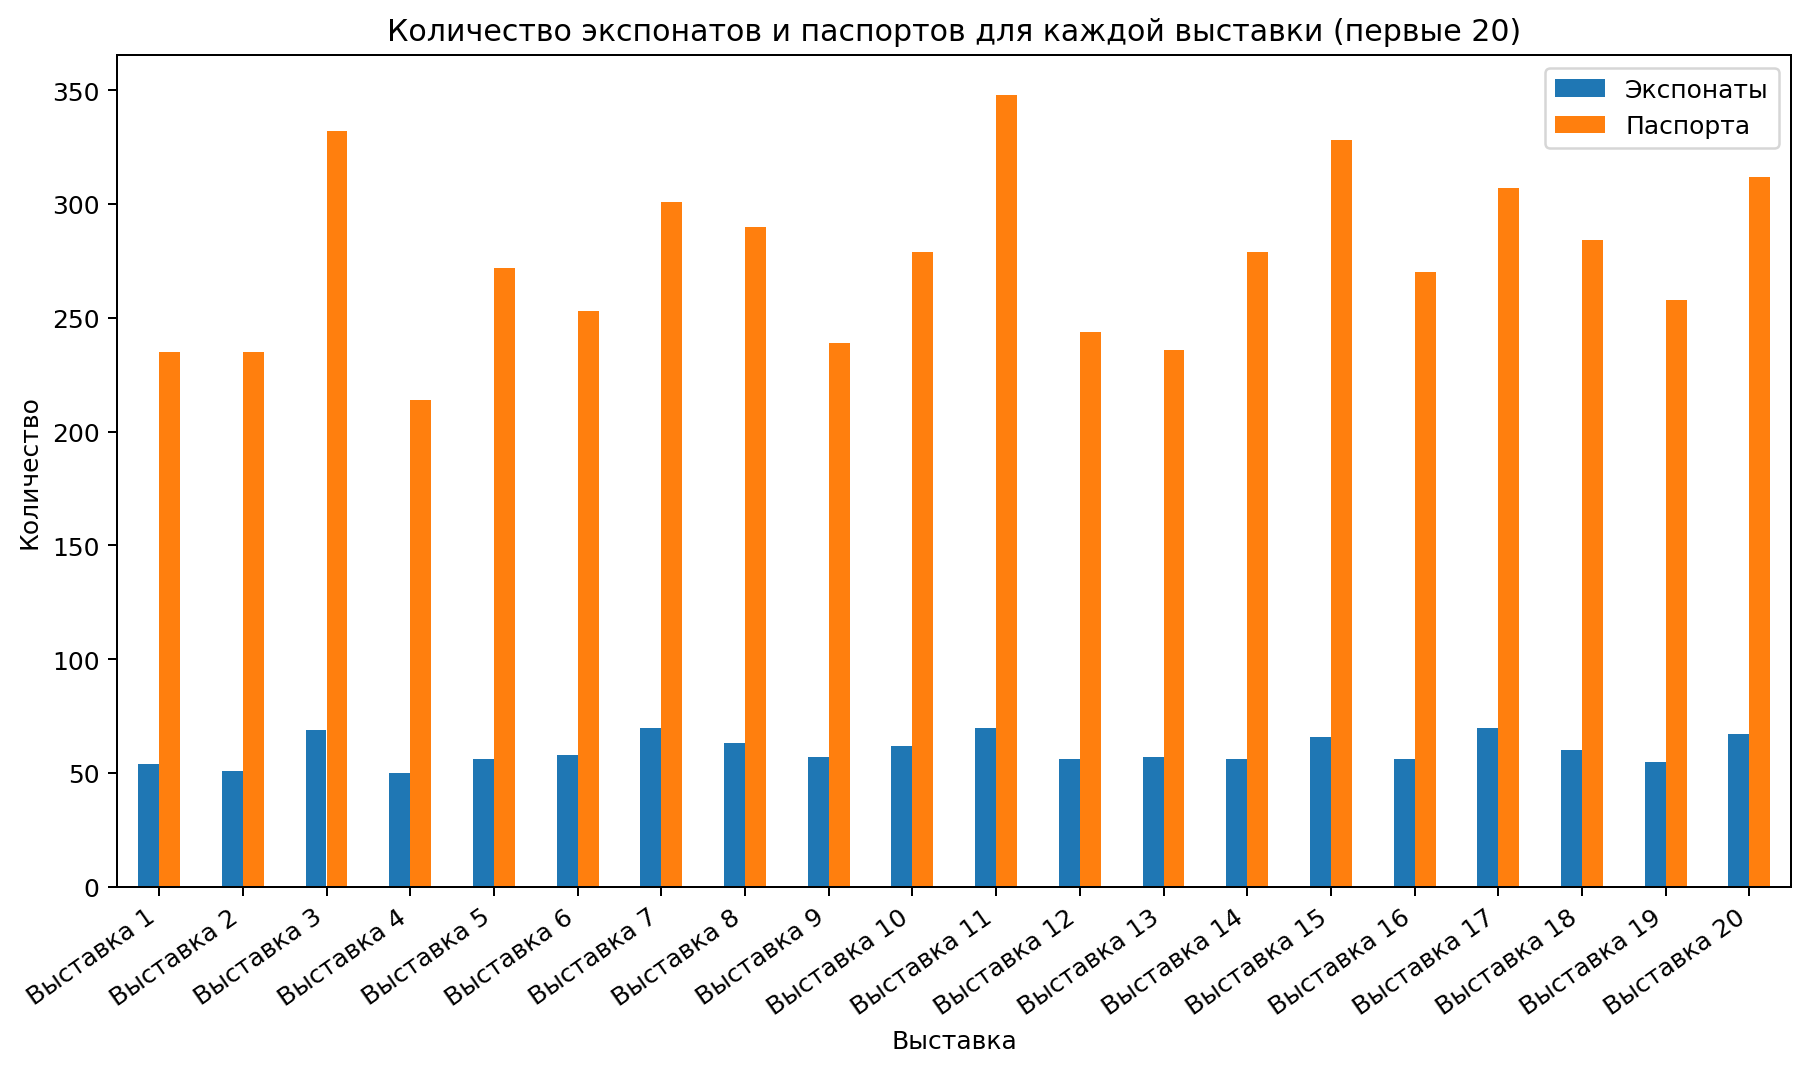
\includegraphics[width=\textwidth,height=14cm, keepaspectratio]{pic/q3_2d_histogram.png}
    \caption{Двумерная гистограмма по результатам запроса 3}
    \label{fig:q3-histogram}
\end{figure}

План выполнения запроса 3 представлен на Рис.\ref{fig:q3-explain}. \par

\begin{figure}[H]
    \centering
    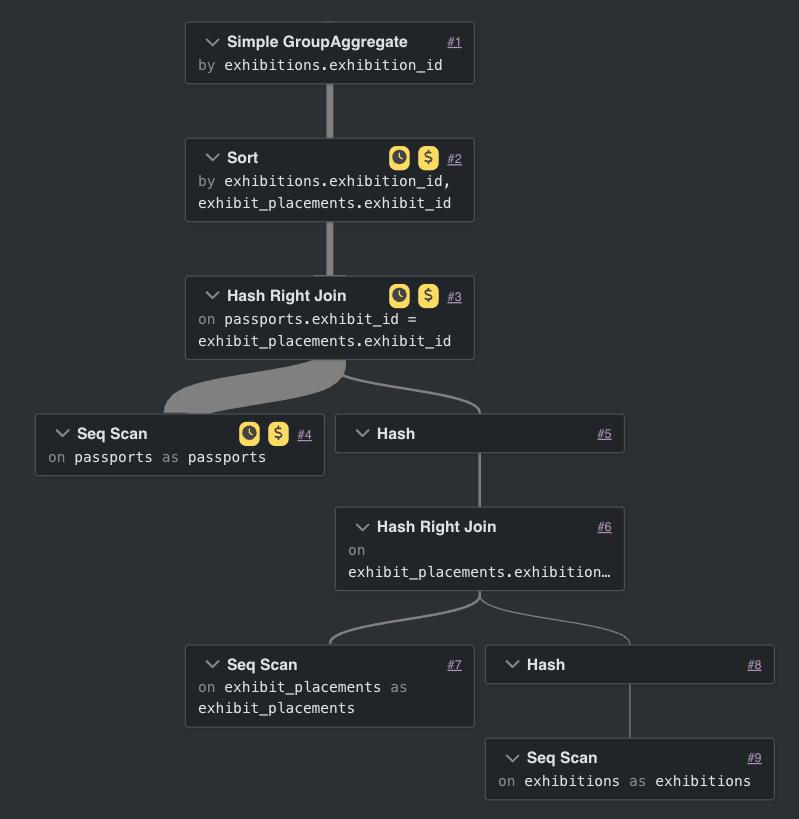
\includegraphics[width=\textwidth,height=12cm,keepaspectratio]{pic/exp3.jpg}
    \caption{План выполнения запроса 3}
    \label{fig:q3-explain}
\end{figure}

План использует внешние соединения, потому что выставка может не иметь размещенных экспонатов, а экспонат может не иметь паспорта. После соединения таблиц выполняется группировка по выставке и два агрегатных подсчета: число различных экспонатов и число различных паспортов. \par

\subsection{Запрос 4.1}

Найти выставочные пространства с максимальным числом выставленных экспонатов. Текст запроса представлен в Листинге~\ref{lst:q41}. \par

\lstinputlisting[language=SQL, caption={Запрос 4.1}, label={lst:q41}, basicstyle=\ttfamily\footnotesize]{../../../queries/q41.sql}

Реляционная формула запроса:
\[
\begin{gathered}
T = 
\gamma_{\substack{\text{exhibition\_space\_id}, \text{room\_type\_name}; \\ \text{COUNT}(\text{exhibit\_id})}}
\left(
\begin{gathered}
\text{exhibition\_spaces} 
\bowtie_{\text{room\_type\_id}} \\
\text{room\_type} 
\bowtie_{\text{exhibition\_space\_id}} \\
\text{display\_places} 
\bowtie_{\text{display\_place\_id}} \\
\text{exhibit\_placements}
\end{gathered}
\right), \\
R_{4.1} = 
\sigma_{\substack{\text{COUNT}(\text{exhibit\_id}) \ = \\ \text{MAX}(\text{COUNT}(\text{exhibit\_id}))}}(T), \\
\text{где } \bowtie \text{ --- это natural join}
\end{gathered}
\]

Результат выполнения запроса 4.1 (выведены первые 20 строк) представлен на Рис.\ref{fig:q41-result}. \par

\begin{figure}[H]
    \centering
    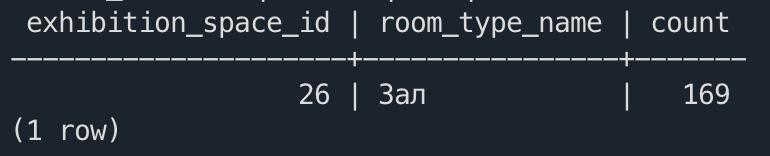
\includegraphics[width=\textwidth,height=2cm,keepaspectratio]{pic/q41.jpg}
    \caption{Результат выполнения запроса 4.1 (выведены первые 20 строк)}
    \label{fig:q41-result}
\end{figure}

План выполнения запроса 4.1 представлен на Рис.\ref{fig:q41-explain}. \par

\begin{figure}[H]
    \centering
    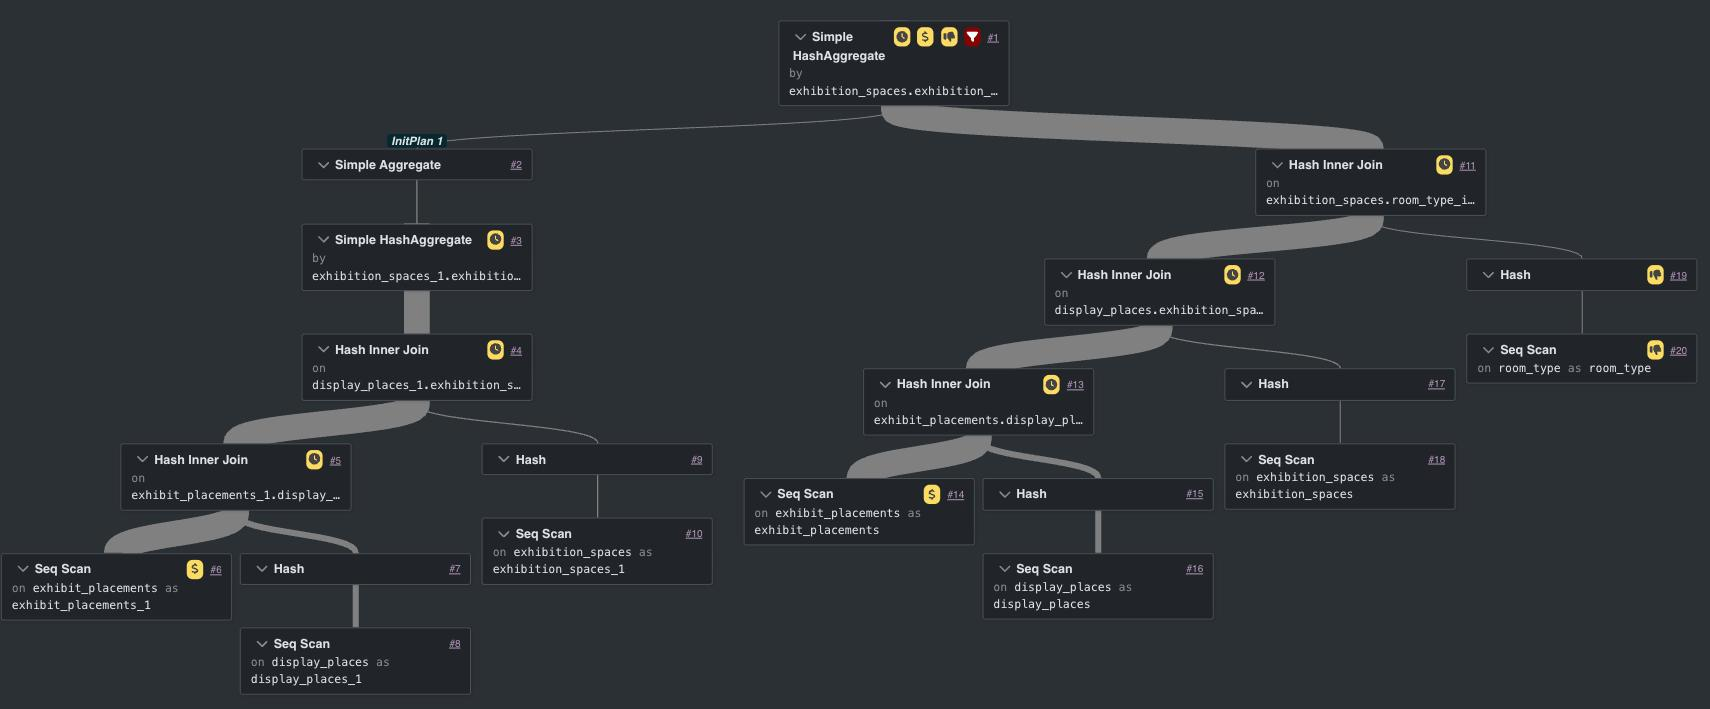
\includegraphics[width=\textwidth,height=0.9\textheight,keepaspectratio]{pic/exp4.1.jpg}
    \caption{План выполнения запроса 4.1}
    \label{fig:q41-explain}
\end{figure}

План строит агрегированную таблицу по выставочным пространствам: соединяет пространства с типами помещений, местами экспонирования и фактами размещения, затем считает число экспонатов. Отдельный подзапрос вычисляет максимальное значение этого счетчика, после чего основной результат фильтруется по равенству максимуму. \par

\subsection{Запрос 4.2}

Найти выставочные пространства с минимальным числом выставленных экспонатов. Текст запроса представлен в Листинге~\ref{lst:q42}. \par

\lstinputlisting[language=SQL, caption={Запрос 4.2}, label={lst:q42}, basicstyle=\ttfamily\footnotesize]{../../../queries/q42.sql}

Реляционная формула запроса:
\[
\begin{gathered}
T = 
\gamma_{\substack{\text{exhibition\_space\_id}, \text{room\_type\_name}; \\ \text{COUNT}(\text{exhibit\_id})}}
\left(
\begin{gathered}
\text{exhibition\_spaces} 
\bowtie_{\text{room\_type\_id}} \\
\text{room\_type} 
\bowtie_{\text{exhibition\_space\_id}} \\
\text{display\_places} 
\bowtie_{\text{display\_place\_id}} \\
\text{exhibit\_placements}
\end{gathered}
\right), \\
R_{4.2} = 
\sigma_{\substack{\text{COUNT}(\text{exhibit\_id}) \ = \\ \text{MIN}(\text{COUNT}(\text{exhibit\_id}))}}(T), \\
\text{где } \bowtie \text{ --- это natural join}
\end{gathered}
\]

Результат выполнения запроса 4.2 (выведены первые 20 строк) представлен на Рис.\ref{fig:q42-result}. \par

\begin{figure}[H]
    \centering
    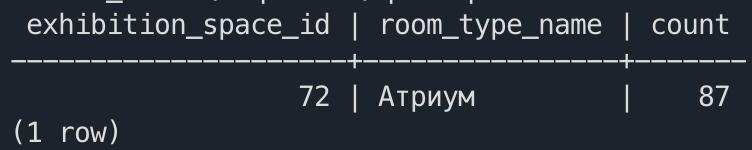
\includegraphics[width=\textwidth,height=2cm,keepaspectratio]{pic/q4.2.jpg}
    \caption{Результат выполнения запроса 4.2 (выведены первые 20 строк)}
    \label{fig:q42-result}
\end{figure}

План выполнения запроса 4.2 представлен на Рис.\ref{fig:q42-explain}. \par

\begin{figure}[H]
    \centering
    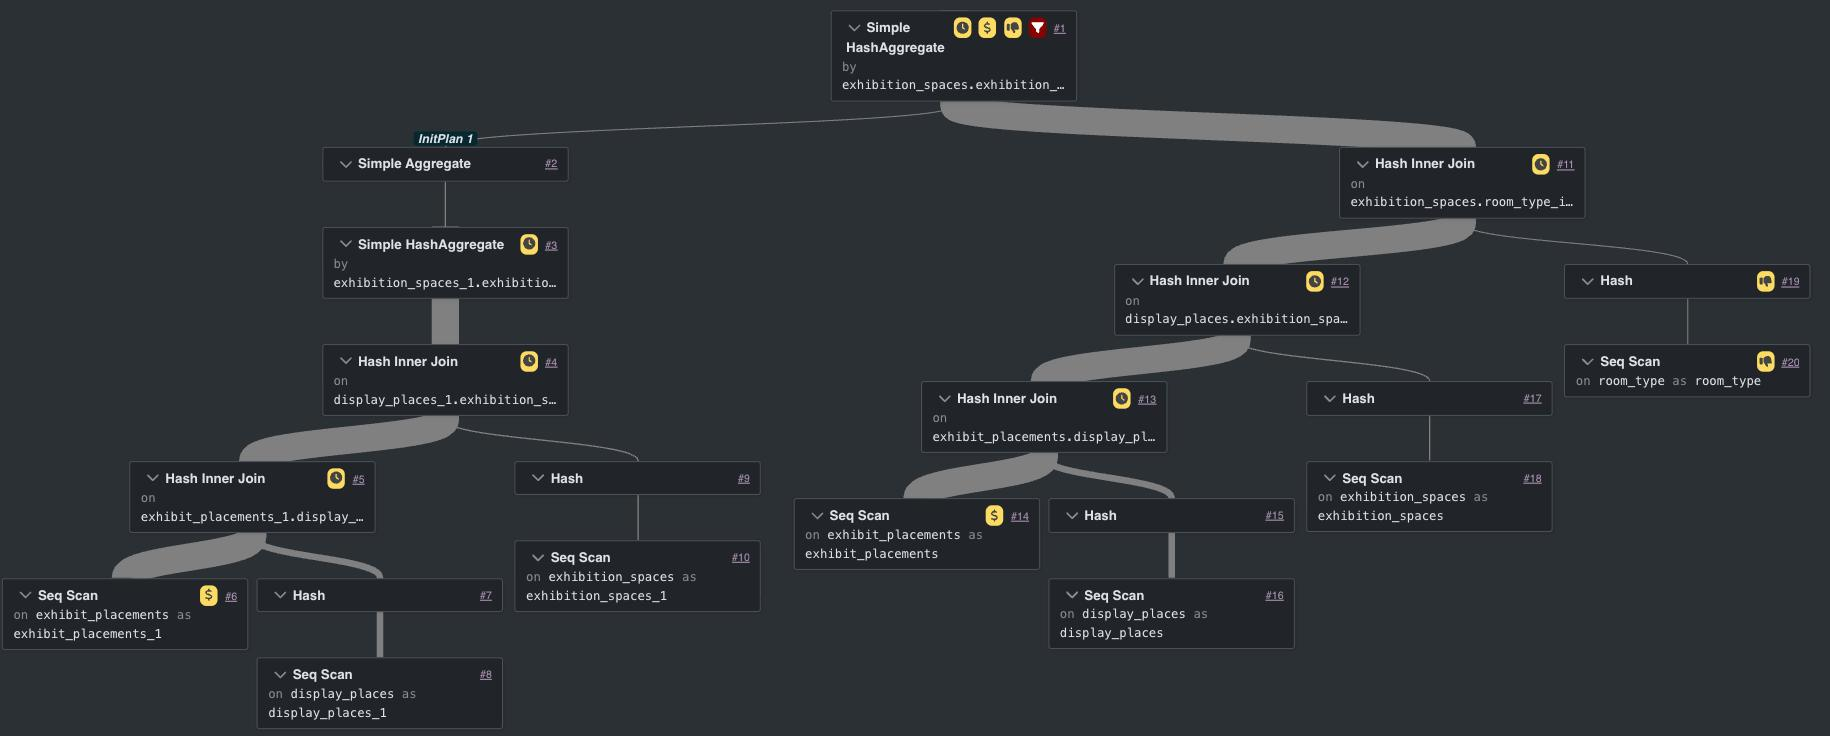
\includegraphics[width=\textwidth,height=0.9\textheight,keepaspectratio]{pic/exp4.2.jpg}
    \caption{План выполнения запроса 4.2}
    \label{fig:q42-explain}
\end{figure}

План аналогичен запросу 4.1: сначала формируется количество размещенных экспонатов по каждому выставочному пространству. Отличие состоит в подзапросе условия HAVING: вместо максимального значения вычисляет минимум, и в итог попадают пространства с минимальным числом экспонатов. \par

\subsection{Запрос 5}

Посчитать число экспонатов с одинаковым числом технических паспортов. Текст запроса представлен в Листинге~\ref{lst:q5}. \par

\lstinputlisting[language=SQL, caption={Запрос 5}, label={lst:q5}, basicstyle=\ttfamily\footnotesize]{../../../queries/q5.sql}

Реляционная формула запроса:
\[
\begin{gathered}
T = 
\gamma_{\substack{\text{exhibit\_id}; \\ \text{COUNT}(\text{passport\_id})}}
\left(
\text{exhibits} \ \bowtie(left)_{\text{exhibit\_id}} \ \text{passports}
\right), \\
R_5 = 
\gamma_{\substack{\text{COUNT}(\text{passport\_id}); \\ \text{COUNT}(\text{exhibit\_id})}}(T), \\
\text{где } \bowtie \text{ --- это natural join}
\end{gathered}
\]

Результат выполнения запроса 5 (выведены первые 20 строк) представлен на Рис.\ref{fig:q5-result}. \par

\begin{figure}[H]
    \centering
    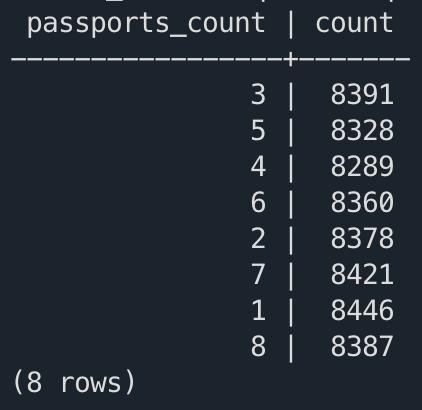
\includegraphics[width=\textwidth,height=7cm,keepaspectratio]{pic/q5.jpg}
    \caption{Результат выполнения запроса 5 (выведены первые 20 строк)}
    \label{fig:q5-result}
\end{figure}

Двумерная гистограмма, построенная по результатам запроса 5, представлена на Рис.\ref{fig:q5-histogram}. \par

\begin{figure}[H]
    \centering
    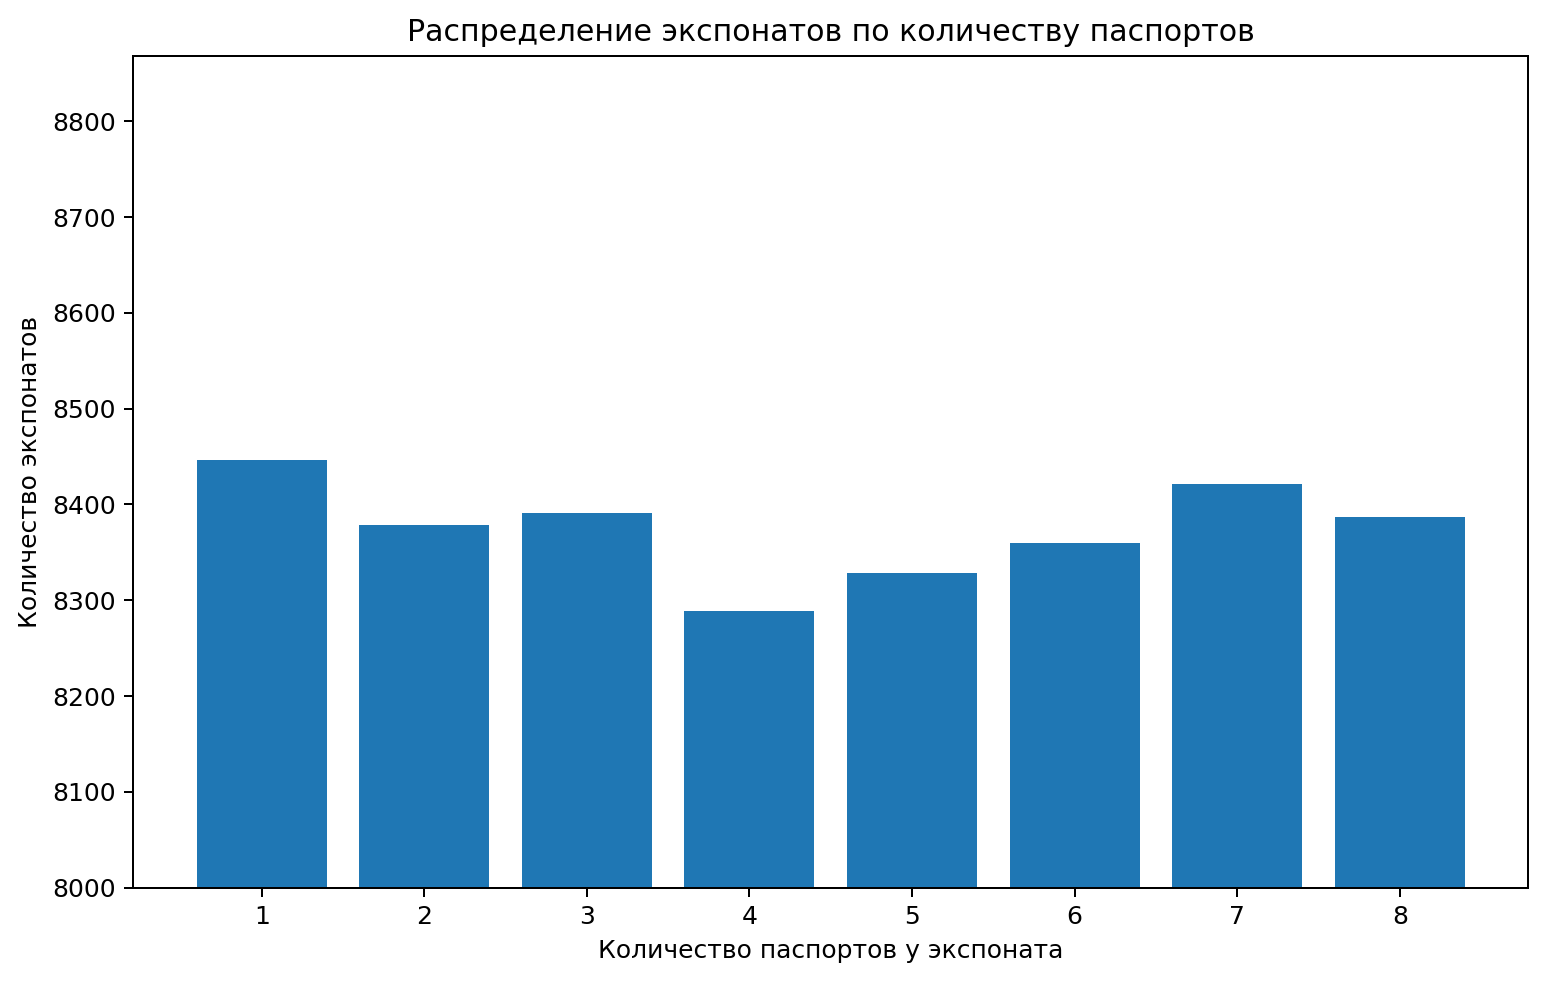
\includegraphics[width=\textwidth,height=0.6\textheight,keepaspectratio]{pic/q5_2d_histogram.png}
    \caption{Двумерная гистограмма по результатам запроса 5}
    \label{fig:q5-histogram}
\end{figure}

План выполнения запроса 5 представлен на Рис.\ref{fig:q5-explain}. \par

\begin{figure}[H]
    \centering
    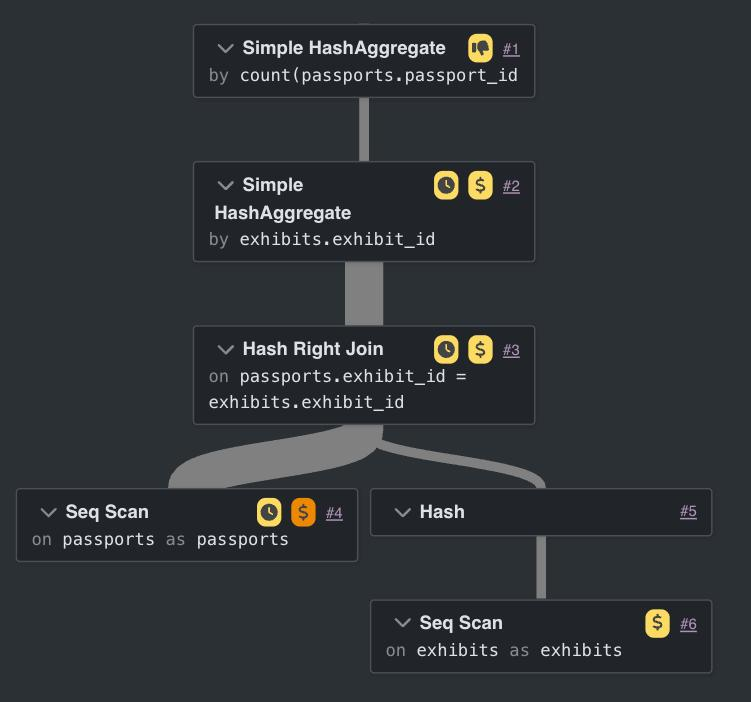
\includegraphics[width=\textwidth,height=0.4\textheight,keepaspectratio]{pic/exp5.jpg}
    \caption{План выполнения запроса 5}
    \label{fig:q5-explain}
\end{figure}

В плане сначала выполняется внешнее соединение экспонатов с паспортами, чтобы учесть в том числе экспонаты без паспортов. Затем подзапрос группирует строки по экспонату и считает паспорта, а внешний запрос группирует уже по полученному числу паспортов и считает количество экспонатов в каждой группе. \par

\subsection{Запрос 6}

Найти выставки, на которых было больше мест экспонирования, чем на выставке А. Текст запроса представлен в Листинге~\ref{lst:q6}. \par

\lstinputlisting[language=SQL, caption={Запрос 6}, label={lst:q6}, basicstyle=\ttfamily\footnotesize]{../../../queries/q6.sql}

Реляционная формула запроса:
\[
\begin{gathered}
T = 
\gamma_{\substack{\text{exhibition\_id}, \text{exhibition\_name}; \\ \text{COUNT}(\text{display\_place\_id})}}
\left(
\begin{gathered}
\text{exhibitions} 
\bowtie_{\text{exhibition\_id}} \\
\text{exhibit\_placements} 
\bowtie_{\text{display\_place\_id}} \\
\text{display\_places}
\end{gathered}
\right), \\
H = 
\gamma_{\text{COUNT}(\text{display\_place\_id})}
\left(
\sigma_{\text{exhibition\_name}=A}
\left(
\text{exhibitions} \ \bowtie_{\text{exhibition\_id}} \ \text{exhibit\_placements}
\right)
\right), \\
R_6 = 
\sigma_{\substack{\text{COUNT}(\text{display\_place\_id}) \ > H}}(T), \\
\text{где } \bowtie \text{ --- это natural join}
\end{gathered}
\]

Результат выполнения запроса 6 (выведены первые 20 строк) представлен на Рис.\ref{fig:q6-result}. \par

\begin{figure}[H]
    \centering
    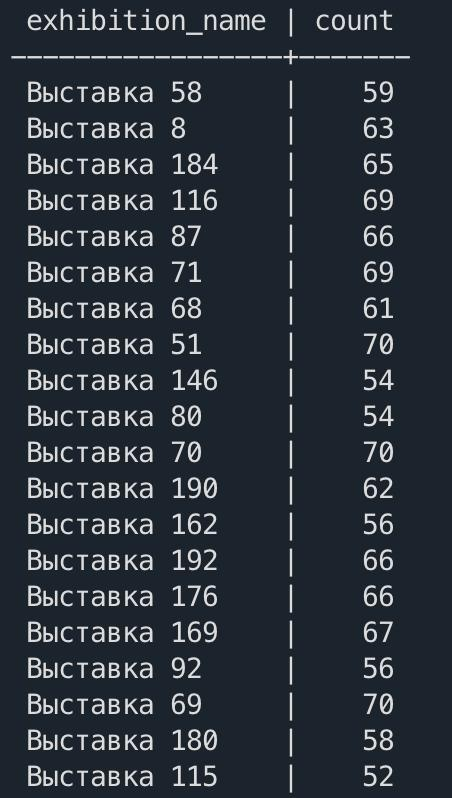
\includegraphics[width=\textwidth,height=10cm,keepaspectratio]{pic/q6.jpg}
    \caption{Результат выполнения запроса 6 (выведены первые 20 строк)}
    \label{fig:q6-result}
\end{figure}

План выполнения запроса 6 представлен на Рис.\ref{fig:q6-explain}. \par

\begin{figure}[H]
    \centering
    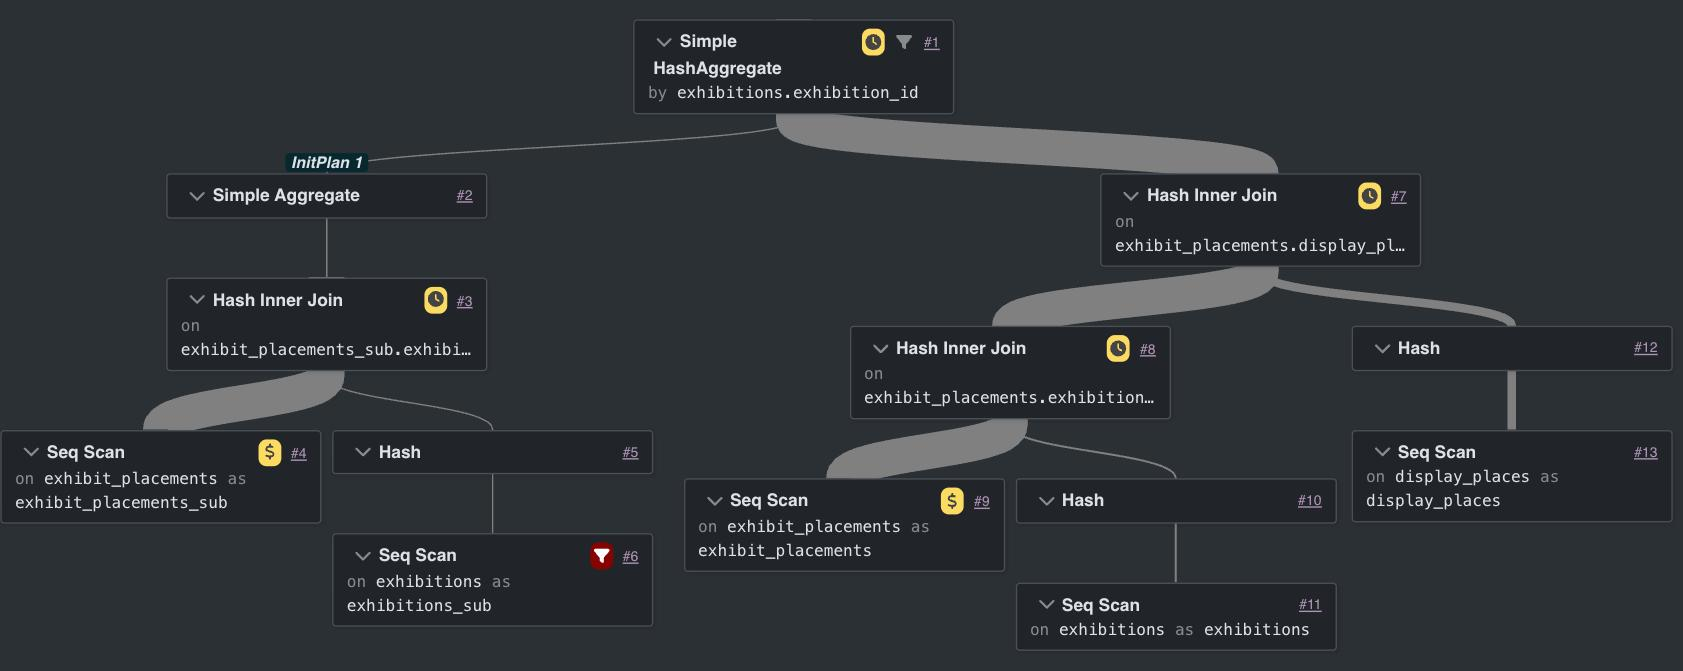
\includegraphics[width=\textwidth,height=0.75\textheight,keepaspectratio]{pic/exp6.jpg}
    \caption{План выполнения запроса 6}
    \label{fig:q6-explain}
\end{figure}

План состоит из двух агрегирующих частей. Подзапрос считает количество мест экспонирования для заданной выставки, а основной запрос считает количество мест для каждой выставки. После группировки применяется условие HAVING, оставляющее только выставки, где количество мест больше значения из подзапроса. \par

\subsection{Запрос 7}

Найти сотрудников, которые ни разу не выставляли ни на одной выставке в качестве кураторов экспонат А. Текст запроса представлен в Листинге~\ref{lst:q7}. \par

\lstinputlisting[language=SQL, caption={Запрос 7}, label={lst:q7}, basicstyle=\ttfamily\footnotesize]{../../../queries/q72.sql}

Реляционная формула запроса:
\[
\begin{gathered}
R_7 = 
\pi_{\text{first\_name}, \text{last\_name}}
\left(
\begin{gathered}
\left(
\text{employees} \ \bowtie_{\text{employee\_id}} \ \text{exhibition\_curators}
\right) - \\ - 
\pi_{\substack{\text{employee\_id}, \\ \text{first\_name}, \\ \text{last\_name}}}
\left(
\sigma_{\text{exhibit\_name}=A}
\left(
\begin{gathered}
\text{employees} \\
\bowtie_{\text{employee\_id}} \\
\text{exhibition\_curators} \\
\bowtie_{\text{exhibition\_id}} \\
\text{exhibitions} \\
\bowtie_{\text{exhibition\_id}} \\
\text{exhibit\_placements} \\
\bowtie_{\text{exhibit\_id}} \\
\text{exhibits}
\end{gathered}
\right)
\right)
\end{gathered}
\right), \\
\text{где } \bowtie \text{ --- это natural join}
\end{gathered}
\]

Результат выполнения запроса 7 (выведены первые 20 строк) представлен на Рис.\ref{fig:q7-result}. \par

\begin{figure}[H]
    \centering
    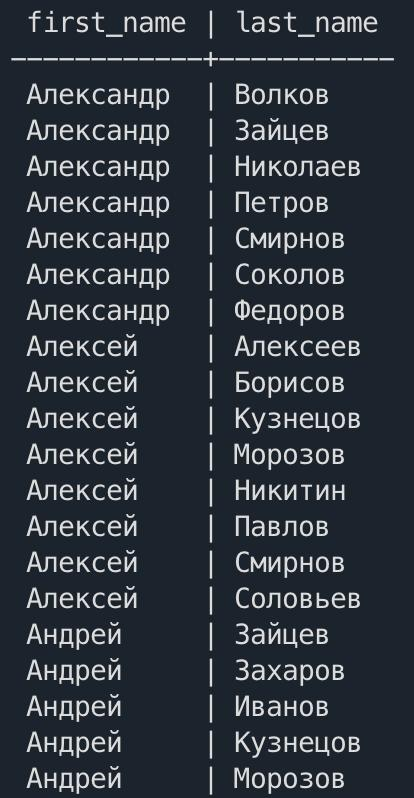
\includegraphics[width=\textwidth,height=8cm,keepaspectratio]{pic/q7.jpg}
    \caption{Результат выполнения запроса 7 (выведены первые 20 строк)}
    \label{fig:q7-result}
\end{figure}

План выполнения запроса 7 представлен на Рис.\ref{fig:q7-explain}. \par

\begin{figure}[H]
    \centering
    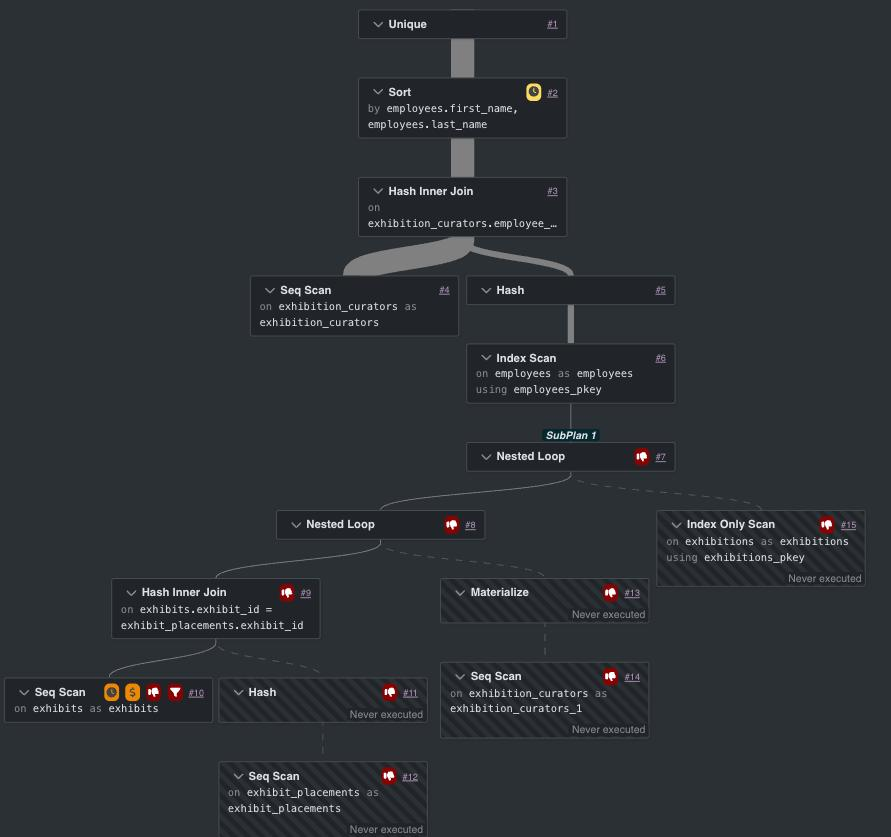
\includegraphics[width=\textwidth,height=0.75\textheight,keepaspectratio]{pic/exp7.jpg}
    \caption{План выполнения запроса 7}
    \label{fig:q7-explain}
\end{figure}

План получает множество сотрудников, которые вообще выступали кураторами, а затем исключает из него сотрудников из подзапроса. Подзапрос находит кураторов выставок, где размещался заданный экспонат. Операция DISTINCT удаляет повторения сотрудников в итоговом результате. \par

\subsection{Запрос 8}

Для каждой выставки и каждого статуса экспоната посчитать число экспонатов. Текст запроса представлен в Листинге~\ref{lst:q8}. \par

\lstinputlisting[language=SQL, caption={Запрос 8}, label={lst:q8}, basicstyle=\ttfamily\footnotesize]{../../../queries/q8.sql}

Реляционная формула запроса:
\[
\begin{gathered}
R_8 = 
\gamma_{\substack{\text{exhibition\_name}, \text{exhibit\_status\_name}; \\ \text{COUNT}(\text{real\_status\_id})}}
\left(
\begin{gathered}
\left(
\text{exhibitions} \times \text{exhibit\_status}
\right) 
\bowtie(left)_{\text{exhibition\_id}} \\
\text{exhibit\_placements} 
\bowtie(left)_{\text{exhibit\_id}} \\
\text{exhibits} 
\bowtie(left)_{\substack{\text{exhibit\_status\_id} \\ \text{exhibit\_status\_name}}} \\
\text{real\_status}
\end{gathered}
\right), \\
\text{где } \bowtie \text{ --- это natural join}
\end{gathered}
\]

Результат выполнения запроса 8 (выведены первые 20 строк) представлен на Рис.\ref{fig:q8-result}. \par

\begin{figure}[H]
    \centering
    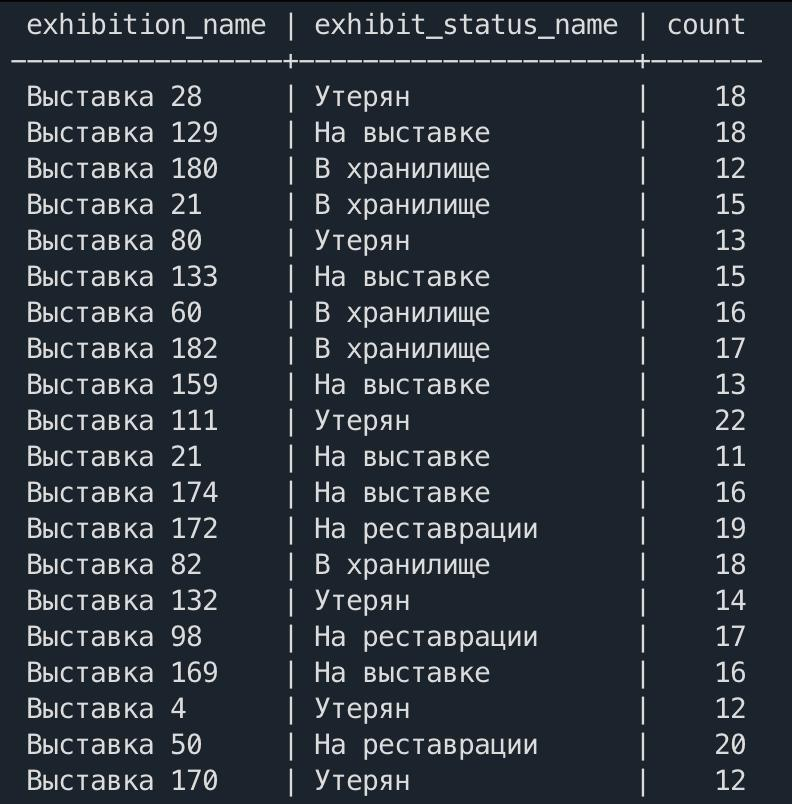
\includegraphics[width=\textwidth,height=0.8\textheight,keepaspectratio]{pic/q8.jpg}
    \caption{Результат выполнения запроса 8 (выведены первые 20 строк)}
    \label{fig:q8-result}
\end{figure}

Трехмерная гистограмма, построенная по результатам запроса 8, представлена на Рис.\ref{fig:q8-histogram}. \par

\begin{figure}[H]
    \centering
    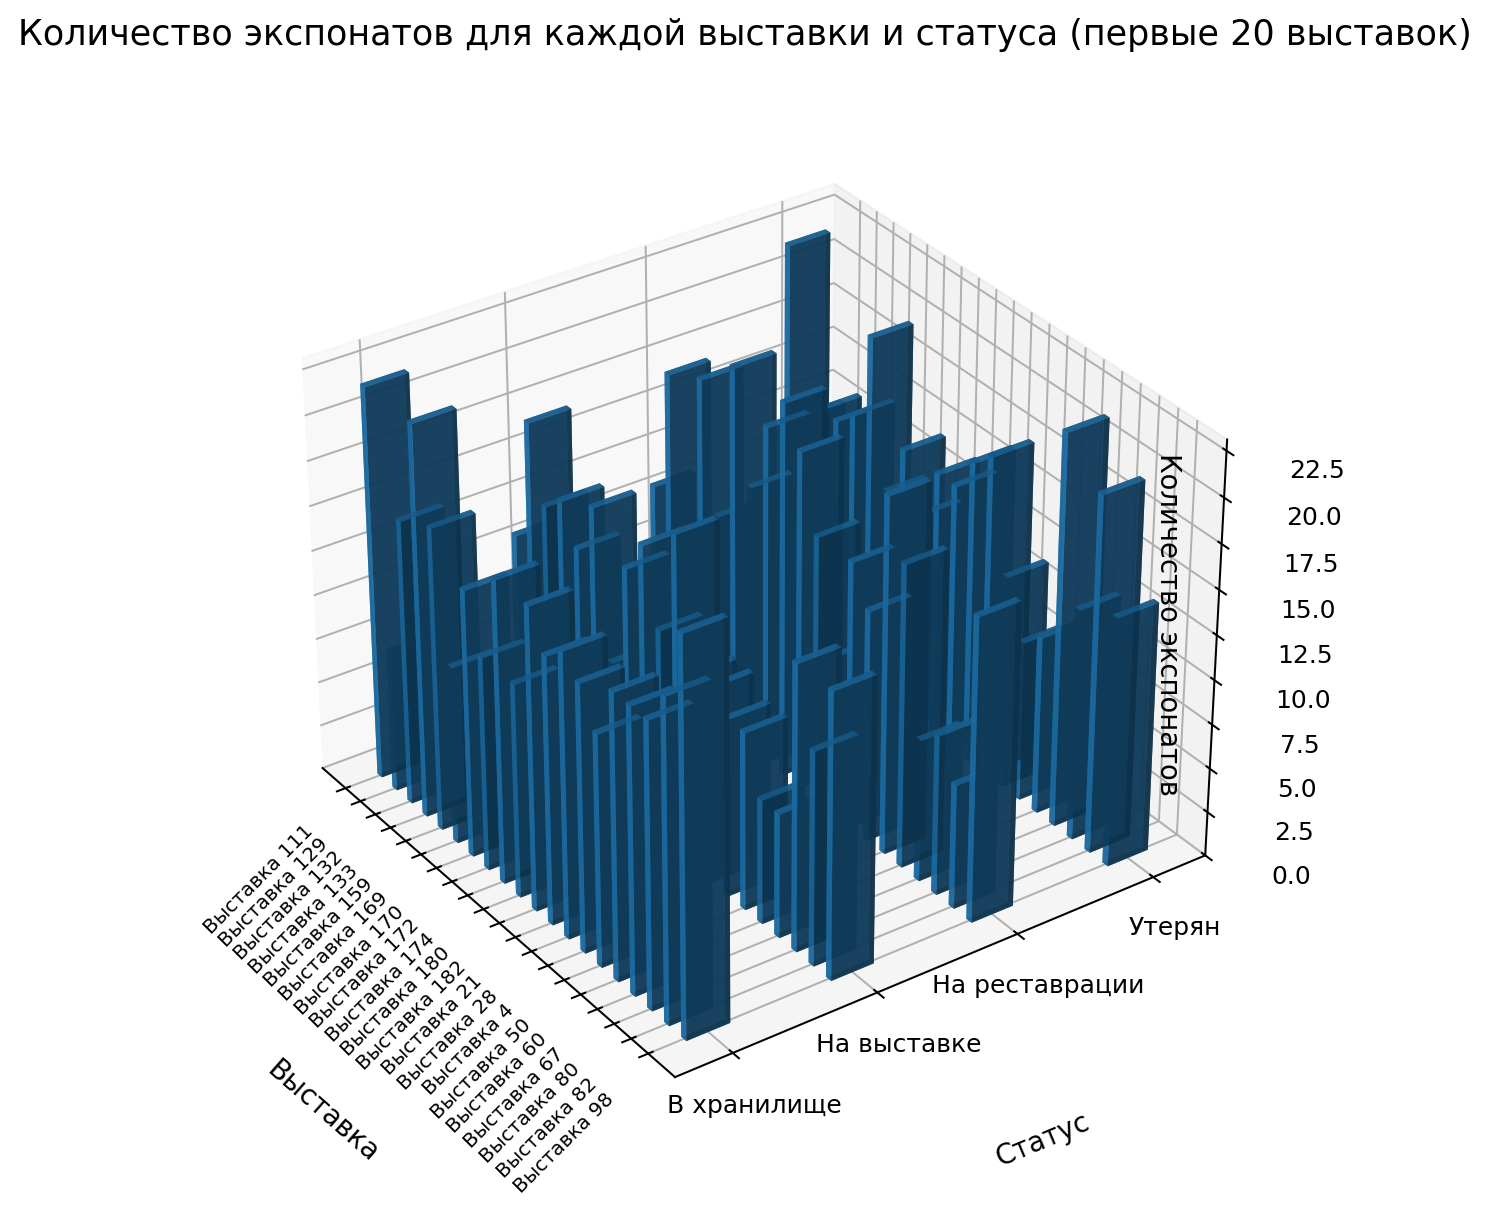
\includegraphics[width=\textwidth,height=0.6\textheight,keepaspectratio]{pic/q8_3d_histogram.png}
    \caption{Трехмерная гистограмма по результатам запроса 8}
    \label{fig:q8-histogram}
\end{figure}

План выполнения запроса 8 представлен на Рис.\ref{fig:q8-explain}. \par

\begin{figure}[H]
    \centering
    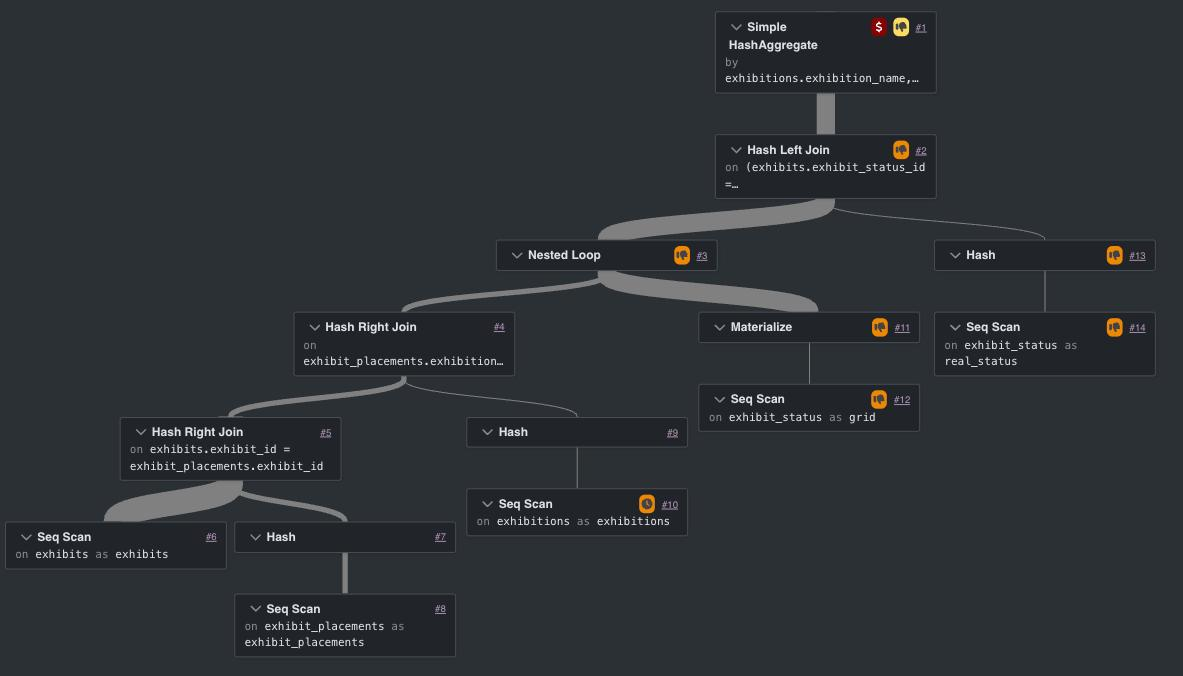
\includegraphics[width=\textwidth,height=0.75\textheight,keepaspectratio]{pic/exp8.jpg}
    \caption{План выполнения запроса 8}
    \label{fig:q8-explain}
\end{figure}

В плане сначала формируется сетка всех пар ``выставка--статус'' с помощью декартова произведения. Затем через внешние соединения добавляются размещения и экспонаты. Последнее соединение со статусом выполнено с дополнительным условием совпадения со строкой сетки, поэтому агрегирование возвращает количество экспонатов для каждой пары выставки и статуса, включая нулевые комбинации. \par

\subsection{Запрос 9}

Для каждого технического паспорта, который составлял сотрудник А, поменять состояние экспоната в паспорте с Б на В. Текст запроса представлен в Листинге~\ref{lst:q9}. \par

\lstinputlisting[language=SQL, caption={Запрос 9}, label={lst:q9}, basicstyle=\ttfamily\footnotesize]{../../../queries/q9.sql}

Реляционная формула запроса:
\[
\begin{gathered}
\text{UPDATE}_{\text{condition\_id} \leftarrow newid} 
\left( 
\text{passports}, 
\right. 
\left.
\sigma_{\text{passport\_id} \in \pi_{\text{passport\_id}}(S)}(\text{passports}) 
\right) \\
 \quad S = 
\sigma_{\substack{\text{last\_name} = A \ \land \\ \text{exhibit\_conditions\_name} = B}}
\left(
\begin{gathered}
\text{passports} 
\bowtie \text{employees} 
\bowtie \text{exhibit\_conditions}
\end{gathered}
\right) \\
newid = 
\pi_{\text{exhibit\_conditions\_id}}
\left(
\sigma_{\text{exhibit\_conditions\_name} = C}(\text{exhibit\_conditions})
\right), \\
\text{где } \bowtie \text{ --- это natural join}
\end{gathered}
\]

Результат выполнения запроса 9 (выведены первые 20 строк) представлен на Рис.\ref{fig:q9-result}. \par

\begin{figure}[H]
    \centering
    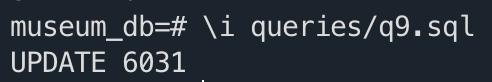
\includegraphics[width=\textwidth,height=2cm,keepaspectratio]{pic/q9.jpg}
    \caption{Результат выполнения запроса 9 (выведены первые 20 строк)}
    \label{fig:q9-result}
\end{figure}

План выполнения запроса 9 представлен на Рис.\ref{fig:q9-explain}. \par

\begin{figure}[H]
    \centering
    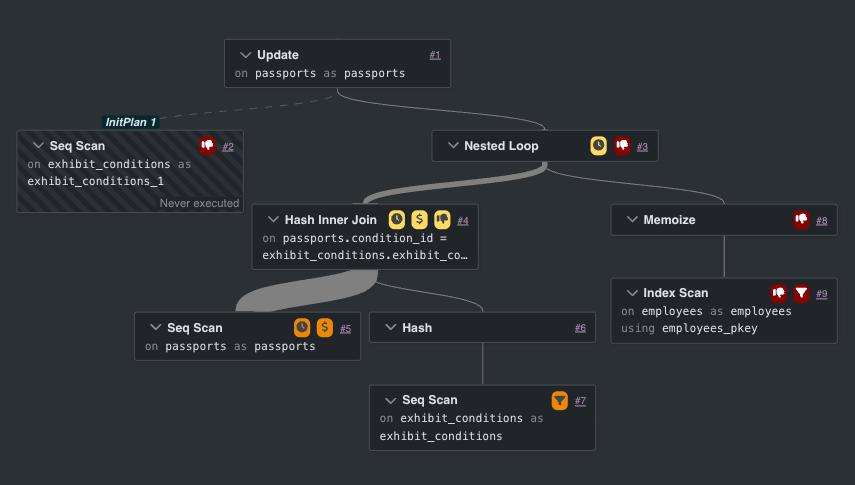
\includegraphics[width=\textwidth,height=0.75\textheight,keepaspectratio]{pic/exp9.jpg}
    \caption{План выполнения запроса 9}
    \label{fig:q9-explain}
\end{figure}

План обновления отбирает паспорта, связанные с сотрудником с заданной фамилией и текущим состоянием экспоната. Подзапрос предварительно получает идентификатор нового состояния по его названию. После отбора строк выполняется операция UPDATE, изменяющая поле \texttt{condition\_id} у найденных технических паспортов. \par

\newpage